\documentclass{standalone}
\usepackage{circuitikz}
\usepackage{amsmath, amssymb}
\usepackage{siunitx}
\begin{document}
	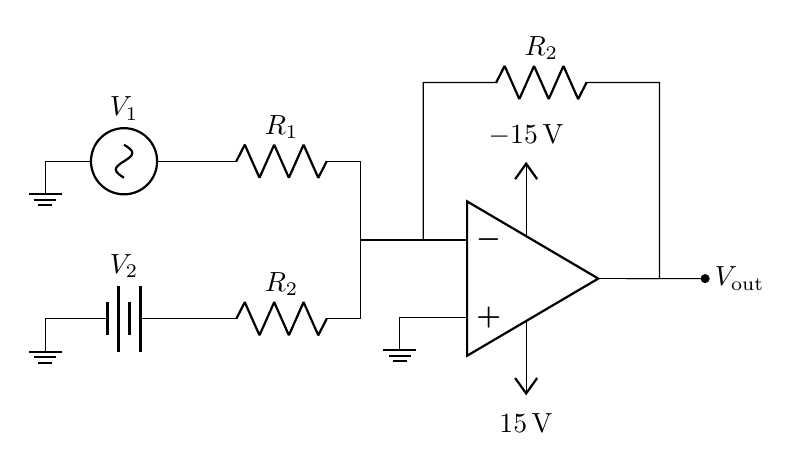
\begin{tikzpicture}
		\draw (0,0) node [op amp] (op) {};
		\draw (op.+) -- ++(-0.5,0) node [ground] {};
		\draw (op.-) -| ++(-1,1) to[R, a=$ R_{1} $] ++(-2,0) to[sV, a=$ V_{1} $] ++(-2,0) node[ground] {};
		\draw (op.-) -| ++(-1,-1) to[R, a=$ R_{2} $] ++(-2,0) to[battery, a=$ V_{2} $] ++(-2,0) node[ground] {};
		\draw (op.up) -- ++(0,0.5) node[vcc]{\SI{-15}{\volt}};
		\draw (op.down) -- ++(0,-0.5) node[vee]{\SI{15}{\volt}};
		\draw (op.-) ++ (-0.2, 0) -- ++(0, 2) to[R, l=$ R_{2} $] ++(3,0)
		|- (op.out);
		\filldraw (op.out) -- ++(1,0) circle [radius=0.05] node[right] {$ V_{\rm out} $};
	\end{tikzpicture}
\end{document}